% Chapter Template

\chapter{Results} % Main chapter title

\label{Chapter4} % Change X to a consecutive number; for referencing this chapter elsewhere, use \cref{ChapterX}

%----------------------------------------------------------------------------------------
%	SECTION 1
%----------------------------------------------------------------------------------------
The results of the different card encodings (MCC Figure \ref{fig:Monte Carlo Control: Q value function with different card encodings} and SARSA Figure \ref{fig:SARSAl: Q value function with different card encodings}) show patterns in the macro range, but no clear pattern can be seen in detail. The macro pattern is explained by the fact that certain card combinations cannot occur and therefore have zero value. As expected, the different card encodings produce different patterns. \\

% \section{Monte Carlo Controll (MCC}
% \newpage

\begin{figure}[ht!]
    \begin{subfigure}{0.5\textwidth}
        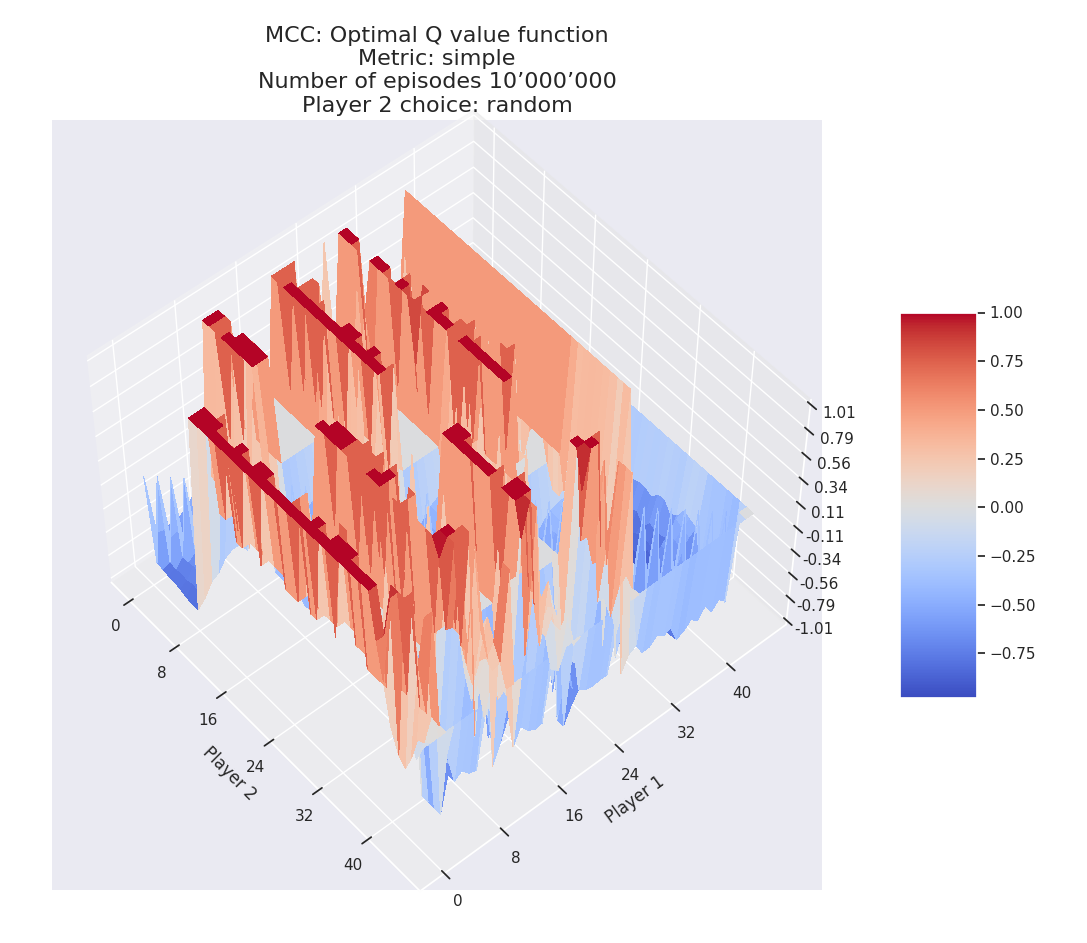
\includegraphics[width=1\linewidth]{Figures/mcc_simple_10000000_random} 
        \caption[Simple]{Simple}
        \label{fig:mccSimple}
    \end{subfigure}
    \begin{subfigure}{0.5\textwidth}
        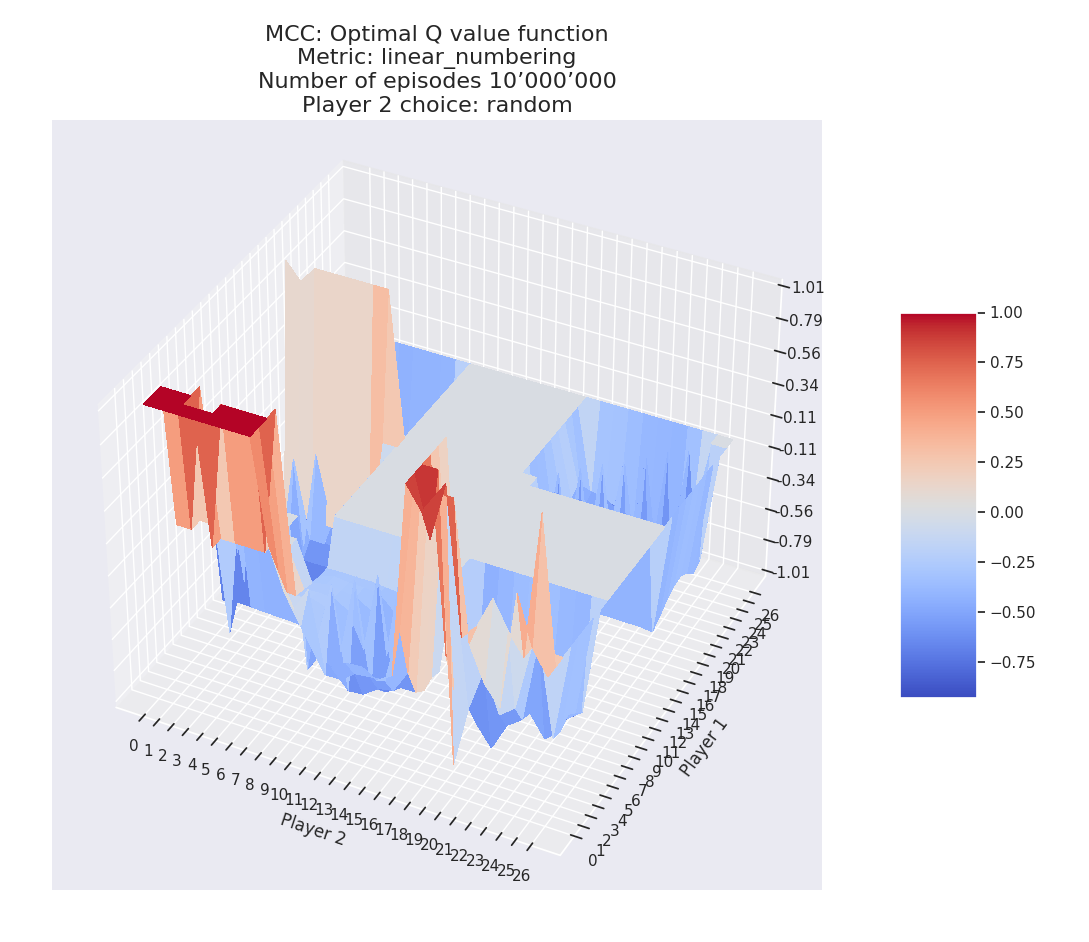
\includegraphics[width=1\linewidth]{Figures/mcc_linear_numbering_10000000_random}
        \caption[Linear Numbering]{Linear Numbering}
        \label{fig:mcclinear numbering}
    \end{subfigure} \\
    \begin{subfigure}{0.5\textwidth}
        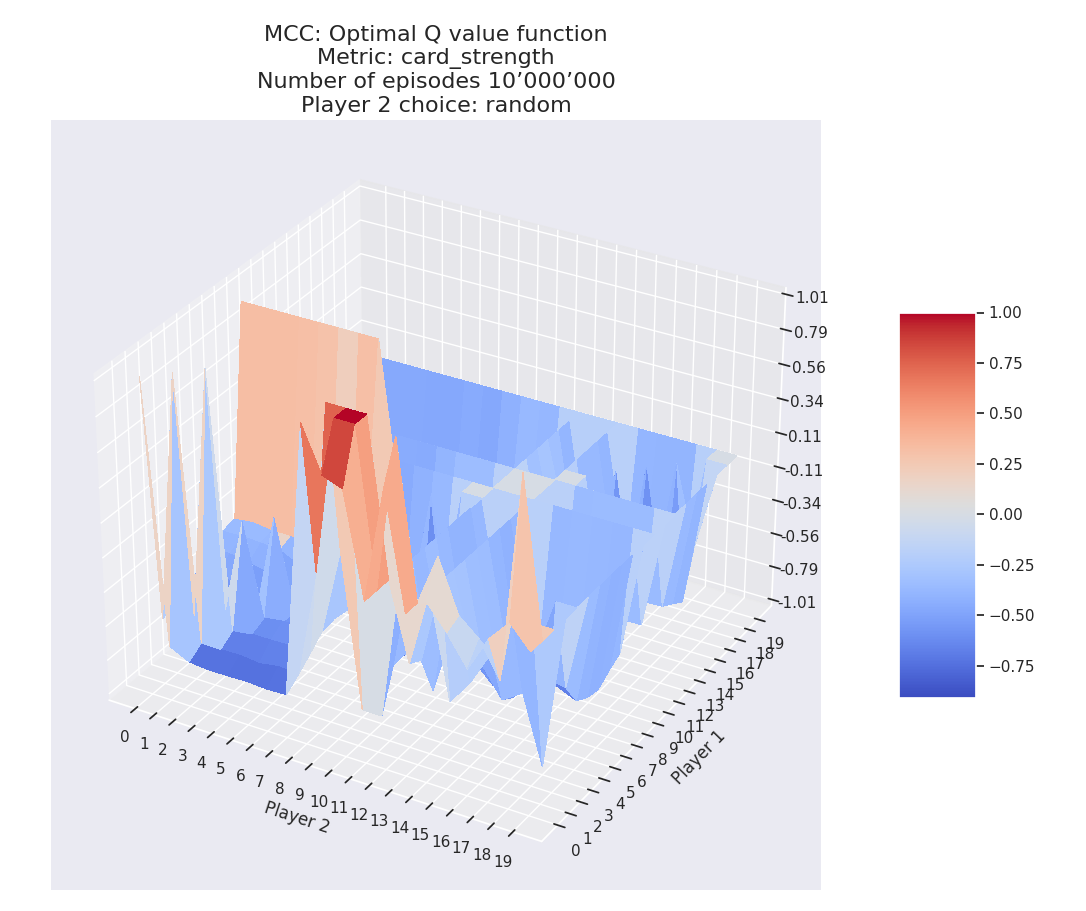
\includegraphics[width=1\linewidth]{Figures/mcc_card_strength_10000000_random}
        \caption[Card Strength]{Card Strength}
        \label{fig:mcccard strength}
    \end{subfigure}
    \begin{subfigure}{0.5\textwidth}
        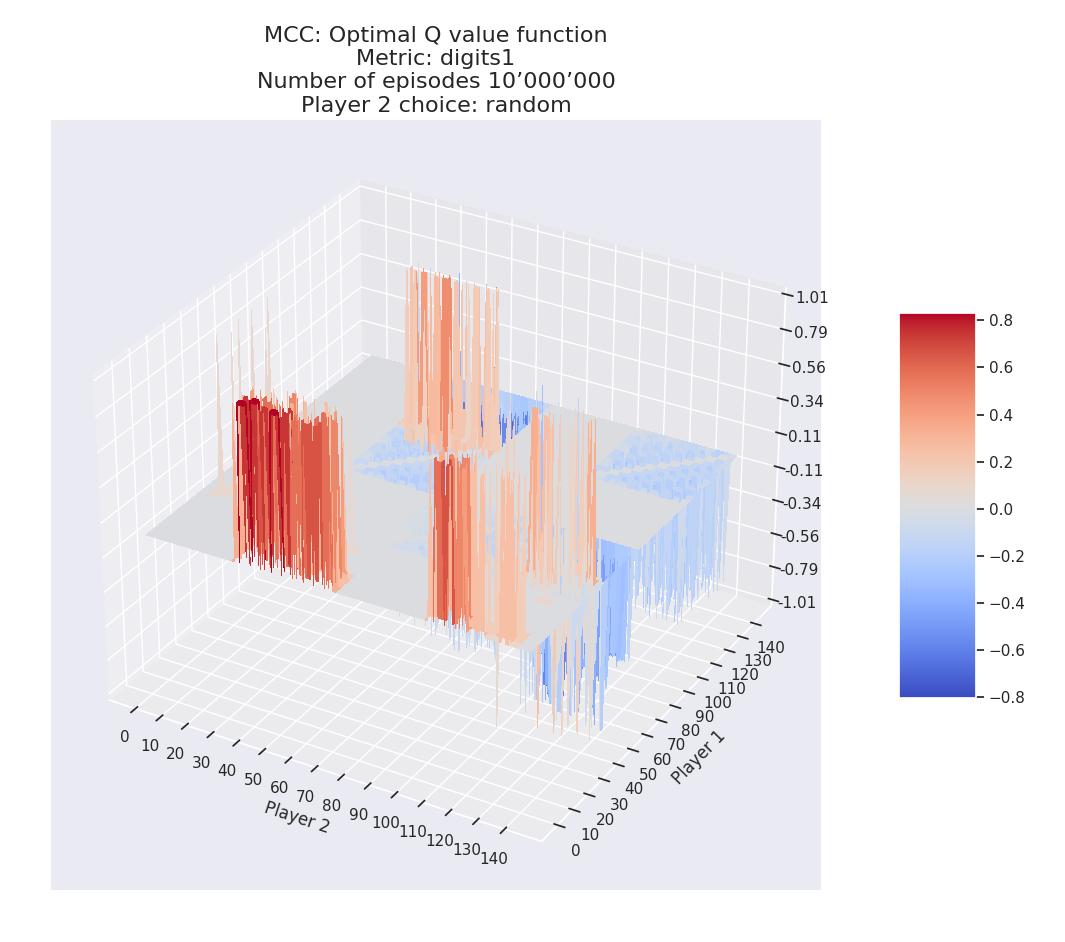
\includegraphics[width=1\linewidth]{Figures/mcc_digits1_10000000_random} 
        \caption[Digits1]{Digits1}
        \label{fig:mccdigits1}
    \end{subfigure} \\
    \begin{subfigure}{0.5\textwidth}
        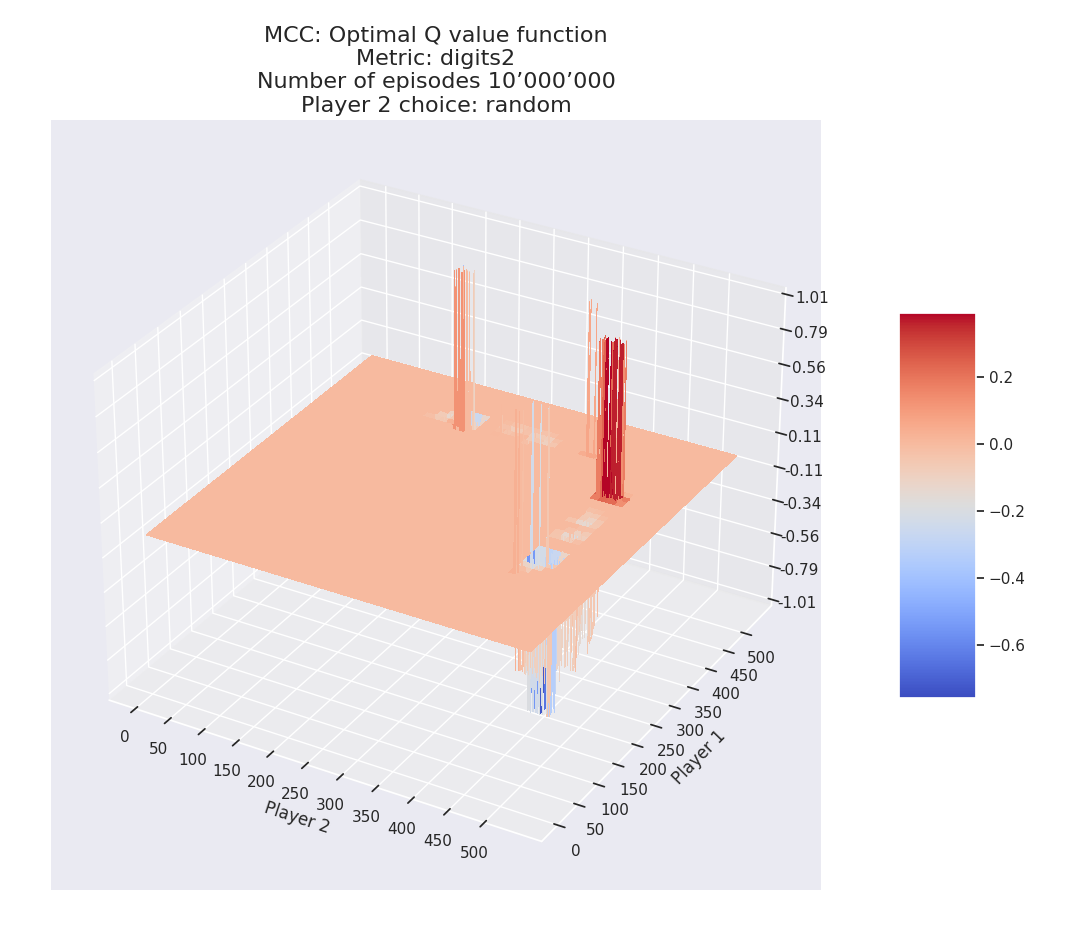
\includegraphics[width=1\linewidth]{Figures/mcc_digits2_10000000_random}
        \caption[Digits2]{Digits2}
        \label{fig:mccdigits2}
    \end{subfigure}
    \caption{Monte Carlo Control: Q value function with different card encodings}
\label{fig:Monte Carlo Control: Q value function with different card encodings}
\end{figure}



% \section{SARSA($ \lambda $)}
% \newpage

\begin{figure}[ht!]
    \begin{subfigure}{0.5\textwidth}
        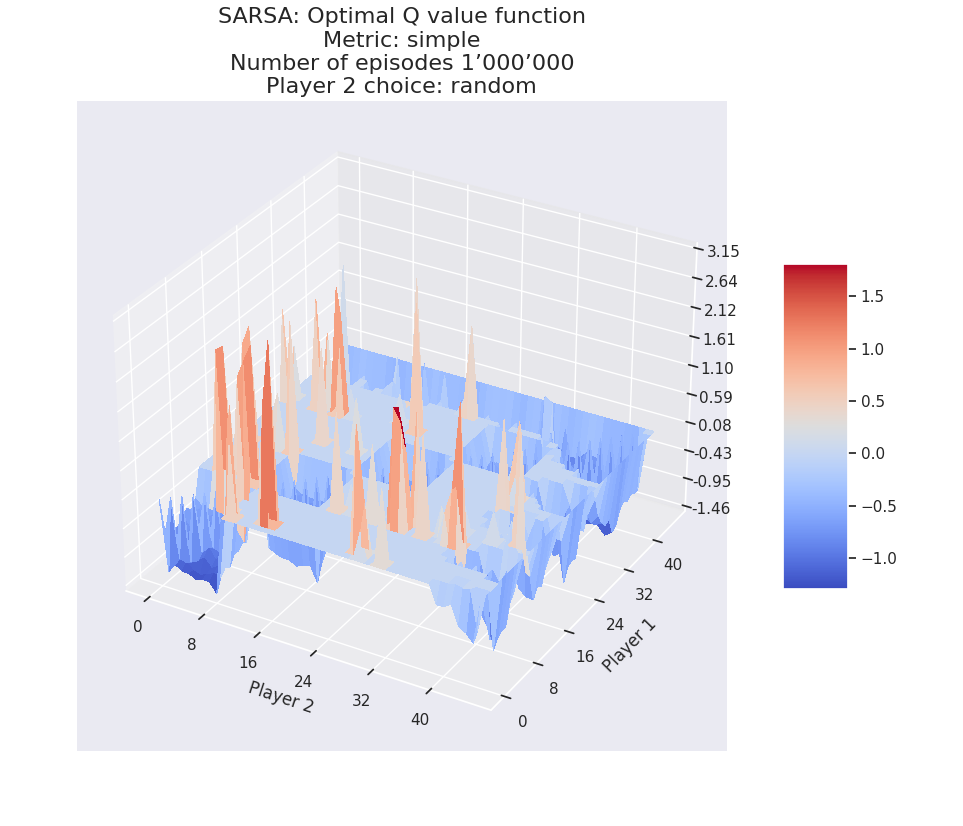
\includegraphics[width=1\linewidth]{Figures/SARSA_simple_1000000_random} 
        \caption[Simple]{Simple}
        \label{fig:SARSASimple}
    \end{subfigure}
    \begin{subfigure}{0.5\textwidth}
        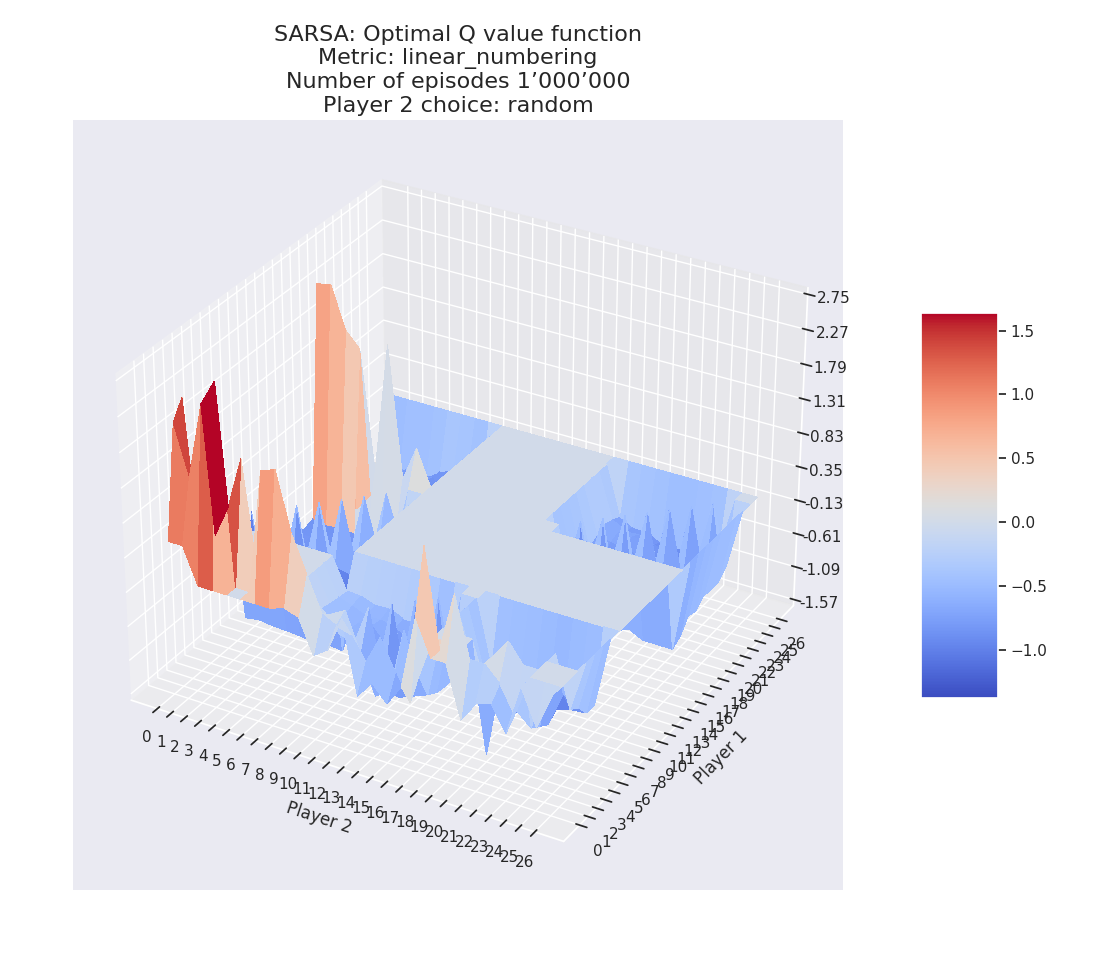
\includegraphics[width=1\linewidth]{Figures/SARSA_linear_numbering_1000000_random}
        \caption[Linear Numbering]{Linear Numbering}
        \label{fig:SARSAlinear numbering}
    \end{subfigure} \\
    \begin{subfigure}{0.5\textwidth}
        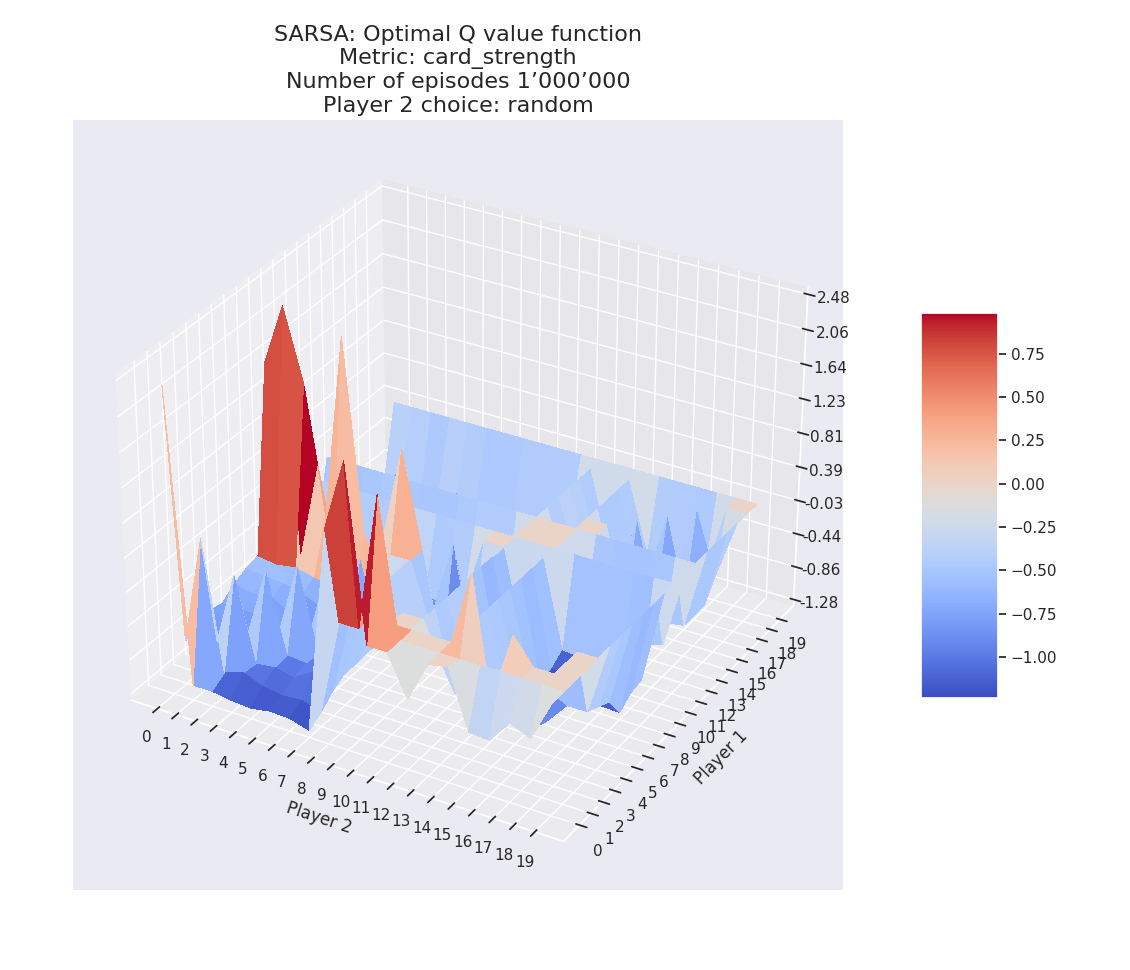
\includegraphics[width=1\linewidth]{Figures/SARSA_card_strength_1000000_random}
        \caption[Card Strength]{Card Strength}
        \label{fig:SARSAcard strength}
    \end{subfigure}
    \begin{subfigure}{0.5\textwidth}
        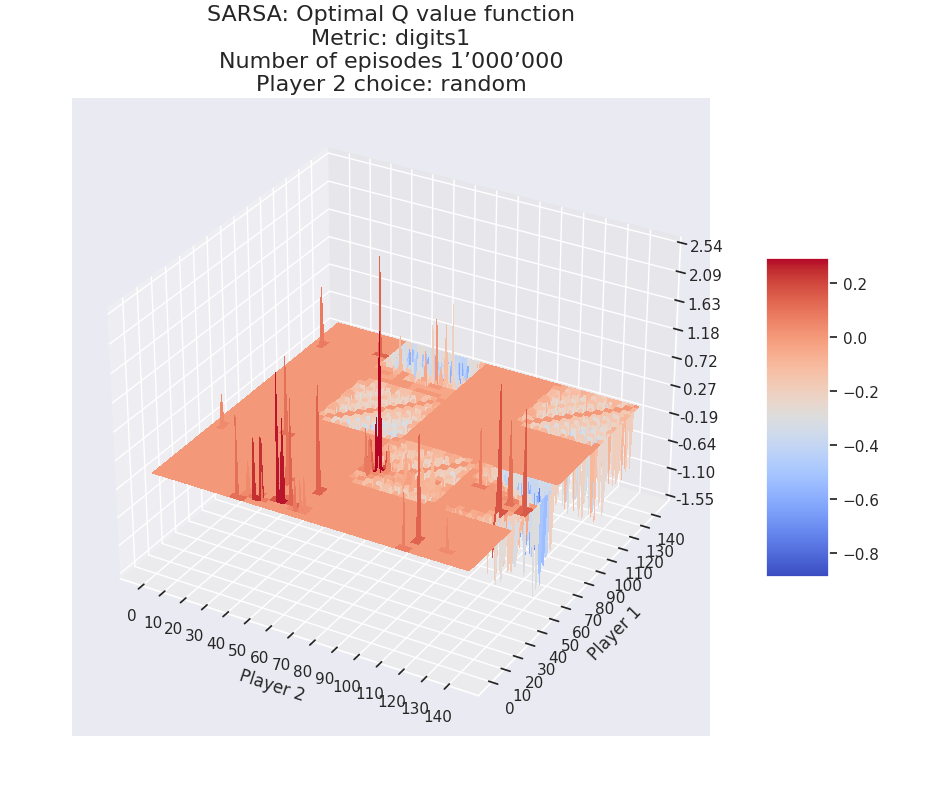
\includegraphics[width=1\linewidth]{Figures/SARSA_digits1_1000000_random} 
        \caption[Digits1]{Digits1}
        \label{fig:SARSAdigits1}
    \end{subfigure} \\
    \begin{subfigure}{0.5\textwidth}
        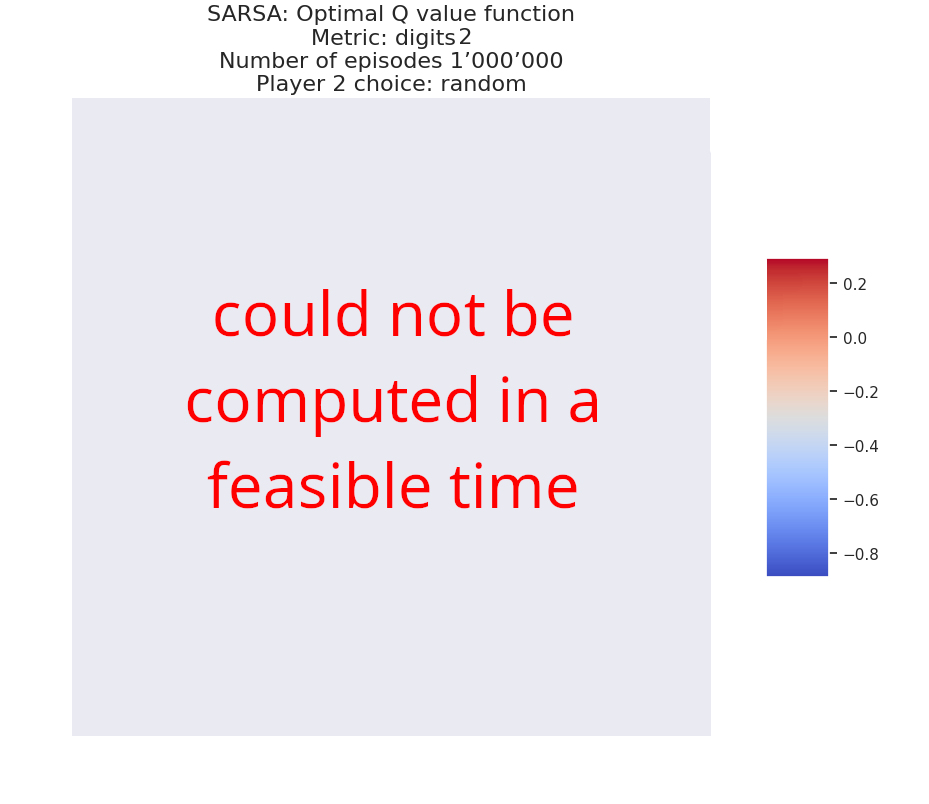
\includegraphics[width=1\linewidth]{Figures/SARSA_digits2_1000000_random}
        \caption[Digits2]{Digits2}
        \label{fig:SARSAdigits2}
    \end{subfigure}
    \caption{SARSA: Q value function with different card encodings}
\label{fig:SARSAl: Q value function with different card encodings}
\end{figure}



\newpage


The two RL algorithms require vastly different execution times. MCC can execute more episodes in less time than SARSA. For the MCC plots, 10 million episodes were used; this was not practical for SARSA since it requires many times more computation time, and also, the card encoding affects the computation times. \\

The two different RL algorithms reveal similar patterns; MCC shows a more uniform Q value function due to the larger number of episodes. However, it can be seen that the SARSA algorythm shows a similar tendency. see Appendix \ref{MCC and SARSA plots side by side with the same card coding} MCC and SARSA plots side by side with the same card encoding\\

The development of the Q value function in dependence on the different numbers of episodes is shown in Figure \ref{fig:Monte Carlo Control: Evolution of Q value function with more episodes}. The greater the number of episodes, the more apparent the pattern. At 100 million episodes, a clear pattern can be seen. \\

\begin{figure}[ht!]
    \begin{subfigure}{0.5\textwidth}
        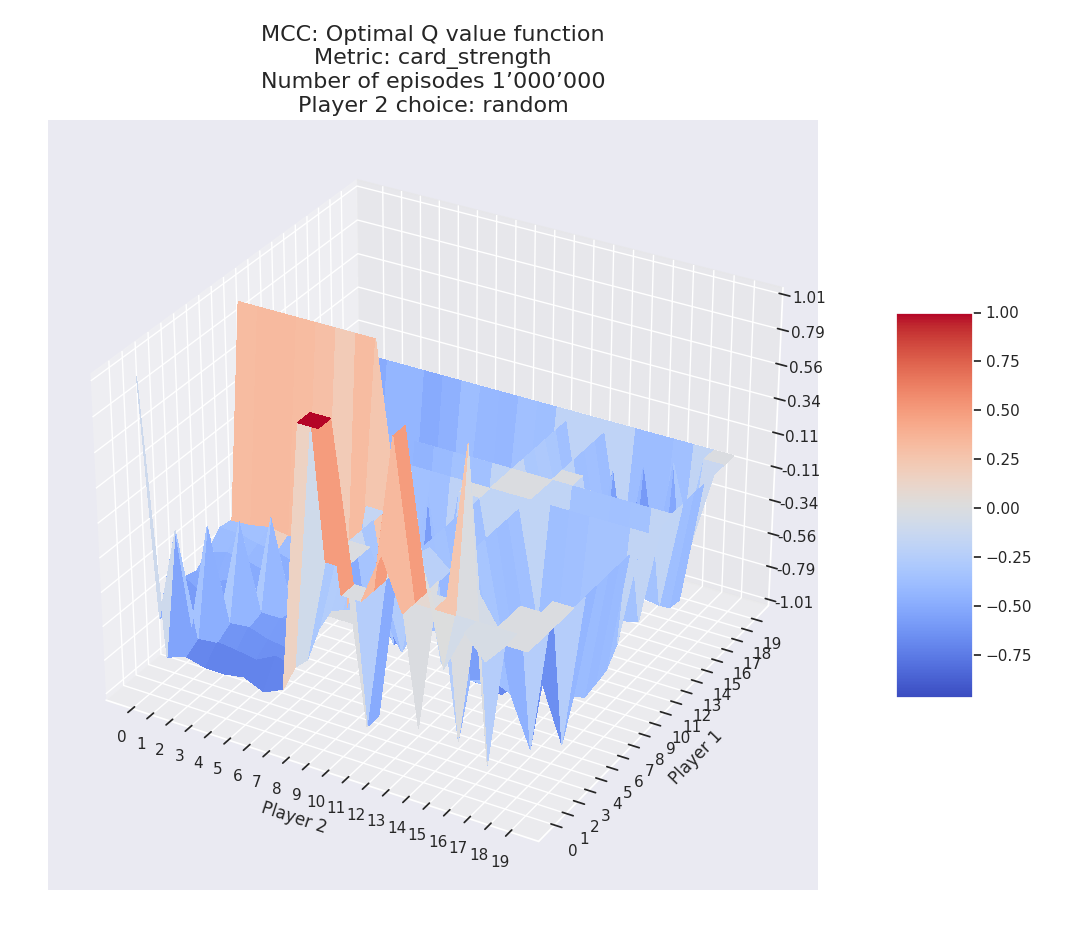
\includegraphics[width=1\linewidth]{Figures/mcc_card_strength_1000000_random} 
        \caption[Card Strength with 1'\,000'\,000 episodes]{Card Strength with 1'\,000'\,000 episodes}
        \label{fig:mcc1}
    \end{subfigure}
    \begin{subfigure}{0.5\textwidth}
        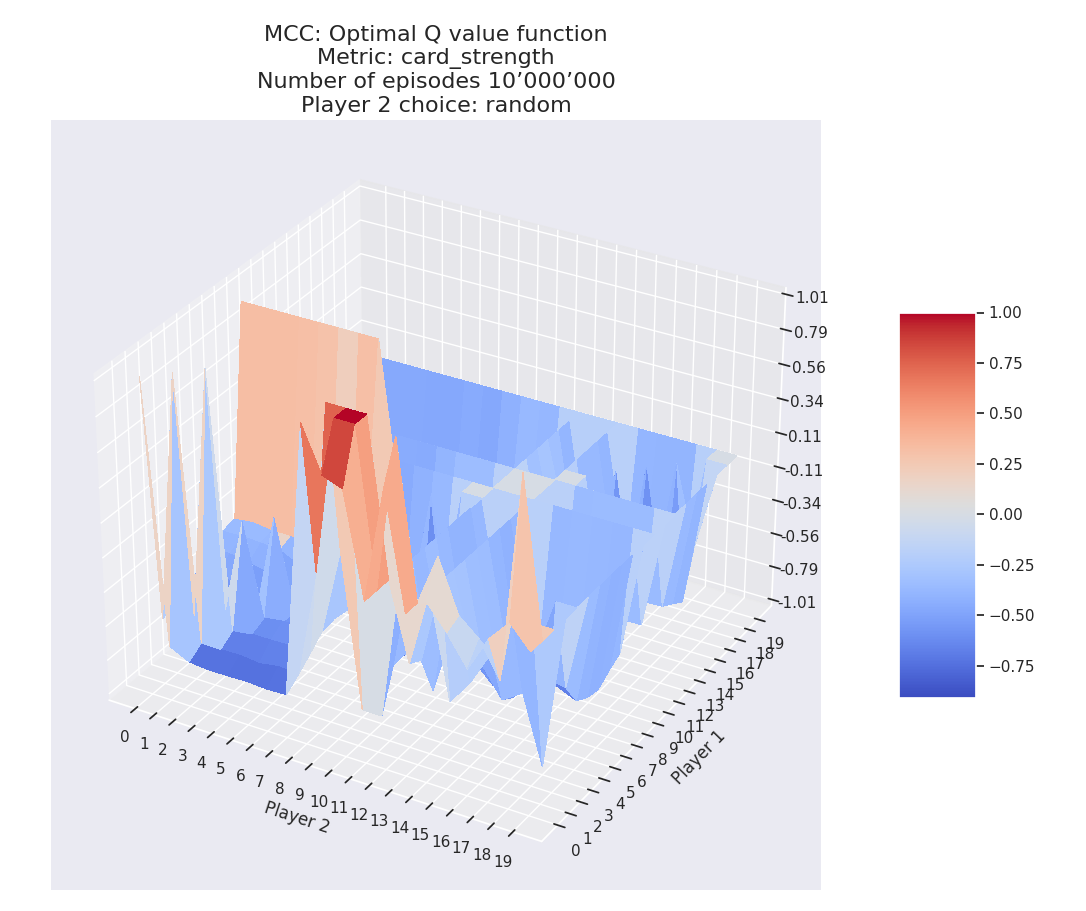
\includegraphics[width=1\linewidth]{Figures/mcc_card_strength_10000000_random}
        \caption[Card Strength with 10'\,000'\,000 episodes]{Card Strength with 10'\,000'\,000 episodes}
        \label{fig:mcc10}
    \end{subfigure} \\
    \begin{subfigure}{0.5\textwidth}
        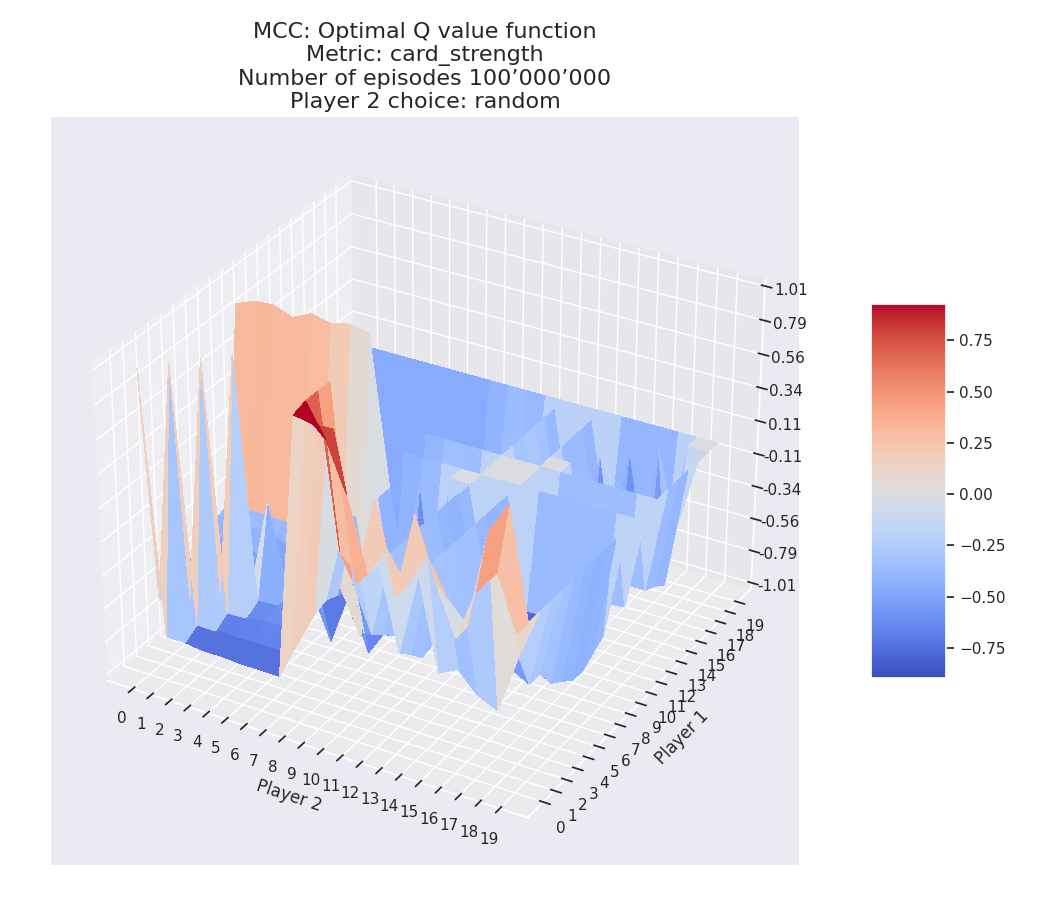
\includegraphics[width=1\linewidth]{Figures/mcc_card_strength_100000000_random}
        \caption[Card Strength with 100'\,000'\,000 episodes]{Card Strength with 100'\,000'\,000 episodes}
        \label{fig:mcc100}
    \end{subfigure}
\caption{Monte Carlo Control: Evolution of Q value function with more episodes}
\label{fig:Monte Carlo Control: Evolution of Q value function with more episodes}
\end{figure}


A comparison with a Q value function where the agent can only randomly select a card shows the same pattern (\ref{fig:Comparison: MCC with different decision options}), confirming that the RL can not demonstrate learning success. This result confirms the "independent" test performed on a second game engine (Jupyter Notebook: dashboard.ipynb, see Github \cite{code}). The test lets two agents play against each other; AGENT 1 uses the learned Q-value function, and AGENT 2 randomly chooses a card. After a million games, AGENT 1 (Q value function) is in the lead with 51\%.


  
\begin{figure}[ht!]
    \begin{subfigure}{0.5\textwidth}
        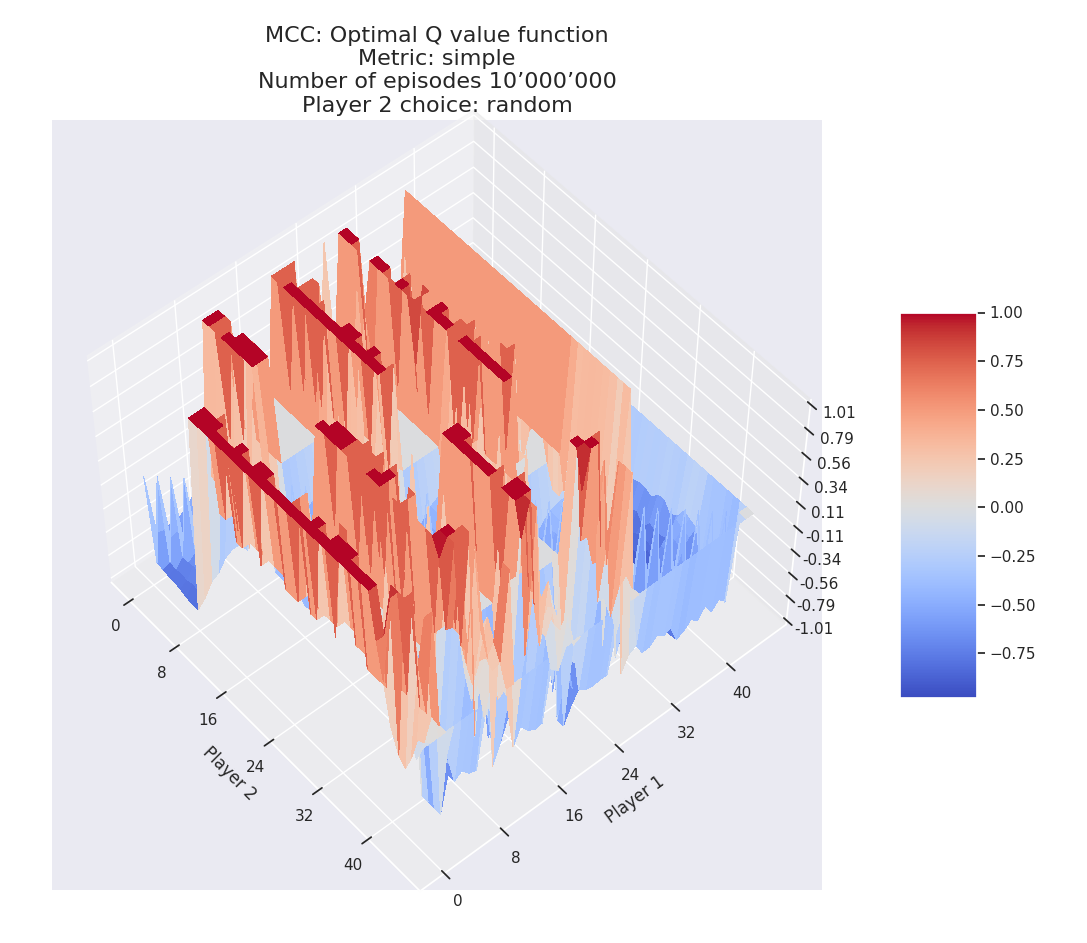
\includegraphics[width=1\linewidth]{Figures/mcc_simple_10000000_random} 
        \caption[RL with options take or leave]{RL with options take or leave}
        \label{fig:RL with options take or leave}
    \end{subfigure}
    \begin{subfigure}{0.5\textwidth}
        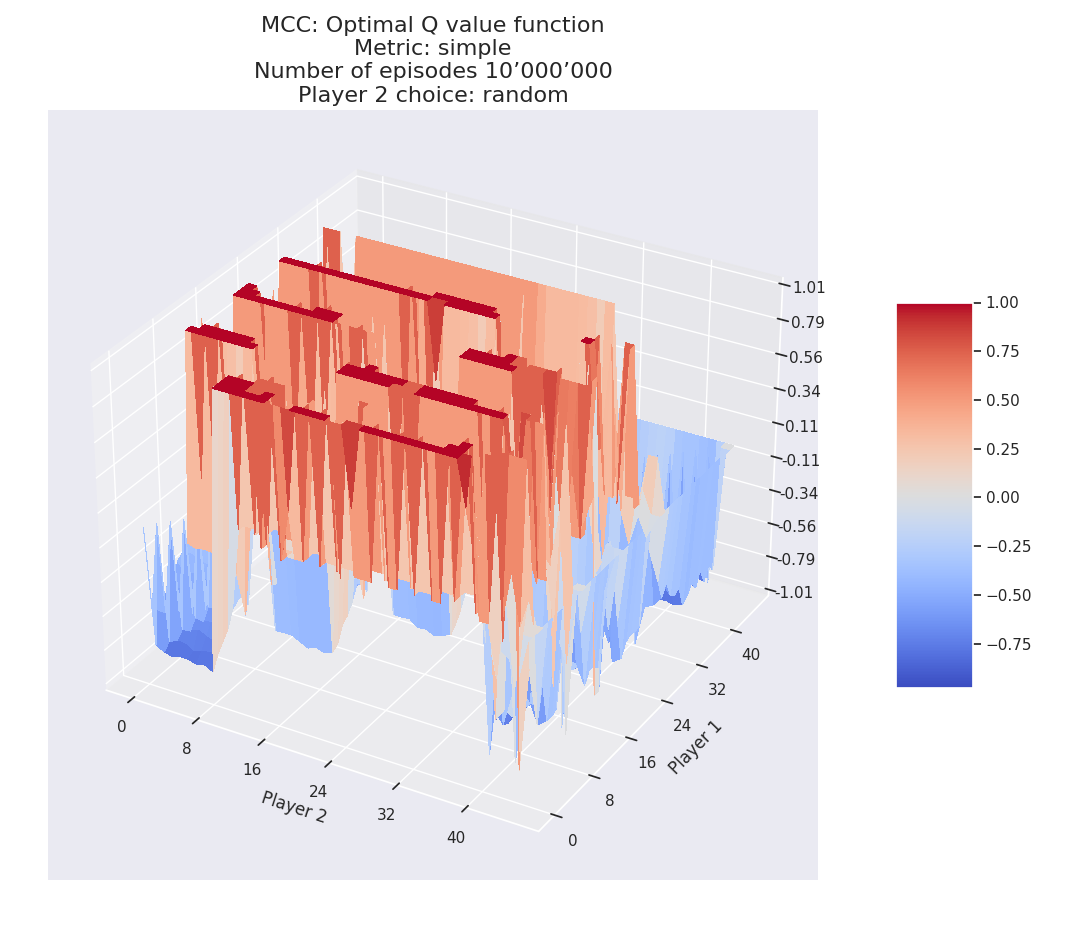
\includegraphics[width=1\linewidth]{Figures/mcc_simple_10000000_random_2}
        \caption[RL with option random]{RL with option random}
        \label{fig:RL with option random}
    \end{subfigure} \\
    \caption{Comparison: MCC with different decision options}
\label{fig:Comparison: MCC with different decision options}
\end{figure}
